\newpage

\backgroundsetup{	scale=1,
				color=black,
				opacity=1,
				angle=0,
				contents={%
 						 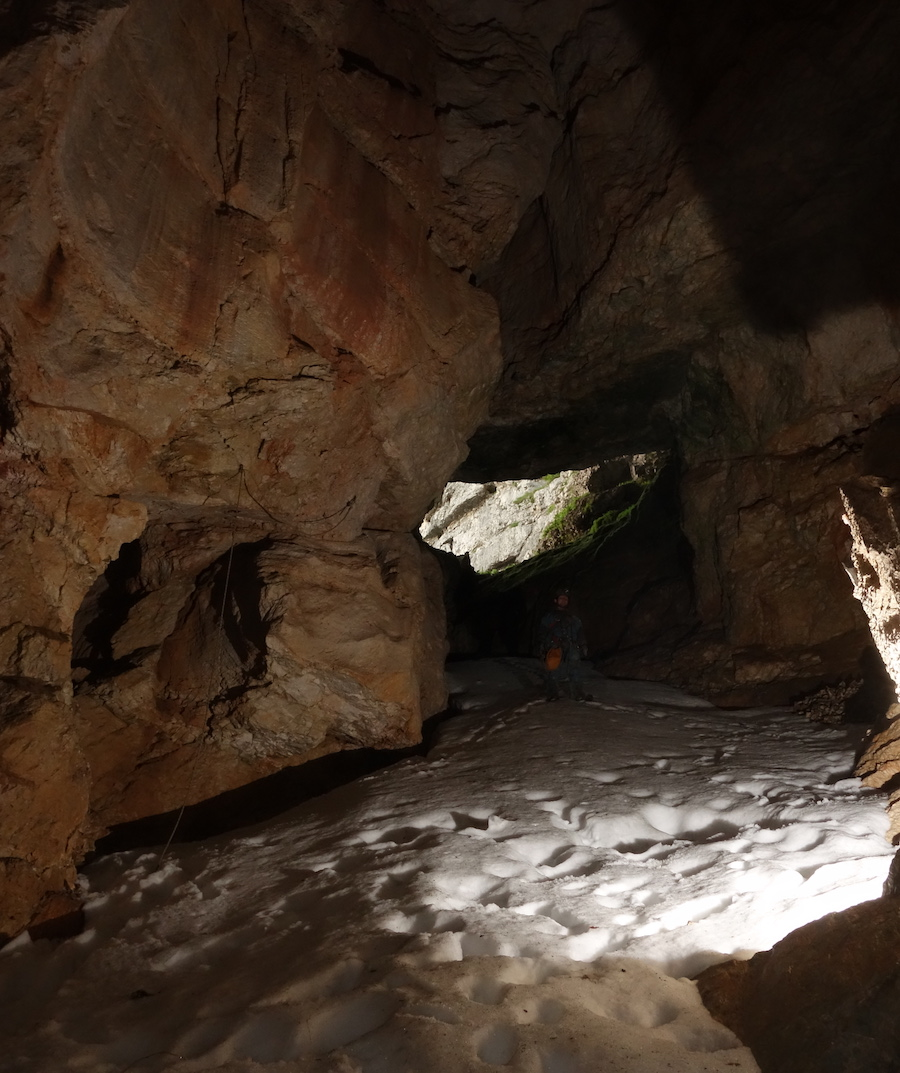
\includegraphics[height=\paperheight]{images/backgrounds/Primadona-2016.jpg}
  				}
	}
\BgThispage

\begin{tcolorbox}
\chapter{2016 - Neprehojene Poti}
	\lettrine{T}{he} exploration target of the Neprehojene Poti expedition to Slovenia was "Primadona", a 750m deep cave with an entrance imposingly 100m down the cliff on the Western side of the Migovec plateau. An impressive 2.6km long cave in its own right, it was connected in to the rest of System Migovec over the winter of 2015/2016 by our partner club the JSPDT. The connection point was between a high level passage in Monatip and the South Eastern end of NCB passage. This means all the major cave systems on the plateau are now connected (until we find more).

	Primadona had been explored sporadically over the preceding decade but mostly with the aim of going deep. The potential for leads relatively close to the surface (within 300m) was a major reason for going, in order that new cavers would have a better chance of doing exploration.

	The exploration was mainly focused in an area known as Rokovo Brezno and over the course of the expedition was pushed 190m deeper and 835m further finally ending in a series of impressively large chambers.  A horizontal passage also connected with the other deep shaft series of Primadona. Higher level leads also brought further 900m of passage, providing more links between Primadona and Monatip through Alkatraz chamber.

	Unfortunately this year was not without incident and one of our party was injured whilst exploring 200m underground. Thanks to the exemplary reaction of all members of the expedition and heroic efforts of the Slovenian cave rescue service he was safely brought to the surface and is now fully recovered.
	\\
	\\
	\\
\end{tcolorbox}